\chapter{Teori}\label{ch:Teori}

I denne opgave er der brugt en række forskellige digitale filtre og redskaber til at implementere en Audio equalizer. De forskellige filtre og redskaber, der er arbejdet med i opgaven er:
\begin{itemize}
\item FIR-filtre
\item IIR-filtre
\item Hanning funktionen
\item Z-transformation
\end{itemize}

\subsection{Equalizer}
En Equalizer er en , den .\\
Equaliseren er blevet implementeret ved at lave 5 forskellige båndpas filtre, der opdeler Audio-signalet i 5 forskellige frekvens dele. Disse båndpas filtre er blevet designet ved brug af IIR- og FIR-filtre. 
Der er et blokdiagram for Equalizeren på figur \ref{fig:Aktivitetsdiagram for Equalizeren}.

\begin{figure}[H]
	\centering
	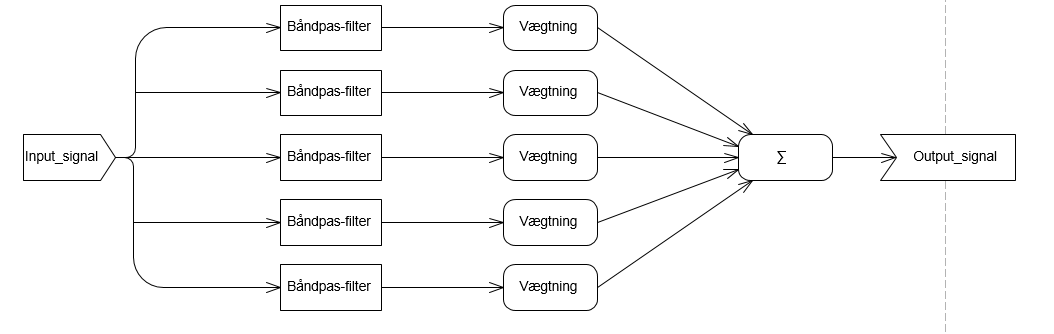
\includegraphics[width=150mm]{figures/Equalizer_flowchart.PNG}
	\caption{Aktivitetsdiagram for Audio Equalizeren}
	\label{fig:Aktivitetsdiagram for Equalizeren}
\end{figure}

Efter signalet er blevet opdelt i 5 forskellige frekvensbånd bliver hver enkelt af frekvens båndene vægtet på forskellige vis.

I det nedenstående afsnit følger en beskrivelse af de to forskellige filtre type. Man kan på nedenstående billede  se den grundlæggende forskel på de to filtre.




\subsection{Z-transformation}
Z-transformationen er en tidsdiskret variant af Laplace Transformation, der transformere et tidsdiskret signal til frekvensdomænet.

Det matematiske udtryk for Z-transformation ses i ligning \ref{eq:Z-transformation}.

\begin{equation}\label{eq:Z-transformation}
{H(z)} = \displaystyle\sum_{n=-\infty }^{\infty} {h(n)z^{-n}}
\end{equation}
 
\subsection{FIR-filtre}
FIR står for Finite Implulse Response, hvilket betyder, at der er et endeligt antal af impulssvar.
Dette kan man se, i ligning \eqref{eq:FIR}, der er diffrensligningen for et FIR filter.
\begin{equation}\label{eq:FIR}
{y(n)} = \displaystyle\sum_{k=0}^{M-1} {b_{k}*x(n-k)}
\end{equation}


\subsection{IIR-filtre}
IIR står for Infinite Impulse Response, hvilket betyder, at det har et uendeligt antal output, da filteret benytter sig af feedback fra tidligere output. Hvis man kigger på ligning \eqref{eq:IIR} kan man se den generelle differensligning for et IIR-filter.


\begin{equation}\label{eq:IIR}
{y(n)} = \displaystyle\sum_{k=0}^{M-1} {b_{k}*x(n-k)}+\displaystyle\sum_{l=1}^{N-1} {a_{l}*y(n-l)}
\end{equation}

x(n): Inputsignal

y(n): Filterets output signal

b_{k}: Filterets feedforward koefficenter

a_{l}: Filterets feedback koefficenter

N-1: filterets orden
\newline
\newline
Fordelen ved et IIR-filter i forhold til et FIR-filter, at de kan bruges til at forstærke et signal, de benytter sig også af færre udregninger og dermed mindre hukommelse. 
Ulemperne ved IIR-filtre er, at de i modsætning til FIR-filtre godt kan være ustabile. 
Dette kan ses af ligning \eqref{eq:IIR overforingsfunktion}, der viser overføringsfunktionen for et IIR-filter i Z-domænet. Ligningnen er fremkommet ved brug af Z-transformationen.

\begin{equation}\label{eq:IIR overforingsfunktion}
{H(z)} =\frac{Y(z)}{X(z)} =\frac{\displaystyle\sum_{k=0}^{N} {b(k)*z^{-k}}}{1-\displaystyle\sum_{k=1}^{M} {a(k)*z^{-k}}}
\end{equation}

Som fremgår af ligning \eqref{eq:IIR overforingsfunktion} indeholder overføringsfunktionen både poler og nulpunkter. Det gælder for IIR-filtre, at de er stabile, hvis alle deres poler har en magnitude, der er mindre end 1 (Polerne lægger i enhedscirklen).

\subsection{Hanning vindue}
Hanning vinduet er en typisk vinduesfunktion med den matematiske funktions foreskrift:
\begin{equation}\label{eq:Hanning}
{w(n)} ={0.5*(1-(\cos \frac{2*\pi*n}{N-1}))}
\end{equation}


Vindues funktioner er er en funktion (værdier), du ganger på dine frekvensbins. Man benytter vindues funktioner til at mindske mængden af lækage, men essensen af en vindues funktin er sådan set bare, at en funktion ganges på en anden funktion. I praksis inden for Digital Signal behandling anvendes stort set altid et Hanning vindue for at undgå lækage.
